%----------------------------------------------------------------------------
\chapter{Manual, future plans and conclusion}
%----------------------------------------------------------------------------
\section{User Manual for the Monitoring system}
The application is a web based application. If it is running it can be opened using a web browser. In production mode the service is listening on the port 8080 of the host computer. In development mode this port number is 9000. Development mode is the default case. If running on localhost, the url should be http://localhost:9000.

If the site is opened a welcome message greets the visitor. There is a short description of the program itself, a short footer at the bottom and a navigation bar at the top of the page. The navigation bar has three elements:
\begin{itemize}
\item \textbf{Sensor browser}, which navigates to the sensor filter page.
\item \textbf{Status}, which shows the results of the last status check of the sensors.
\item \textbf{Help} shows the initial page.
\end{itemize}
By clicking the elements the user will be redirected to the pages accordingly.

\subsection{Sensor browser page}
This page gives an overview of all the sensors that exist in the system. A list can be seen on the page, and after clicking the details of the selected sensor is shown. A screenshot of the page can be seen on Figure \ref{fig:shbrowser}.

\begin{figure}[h]
\centering
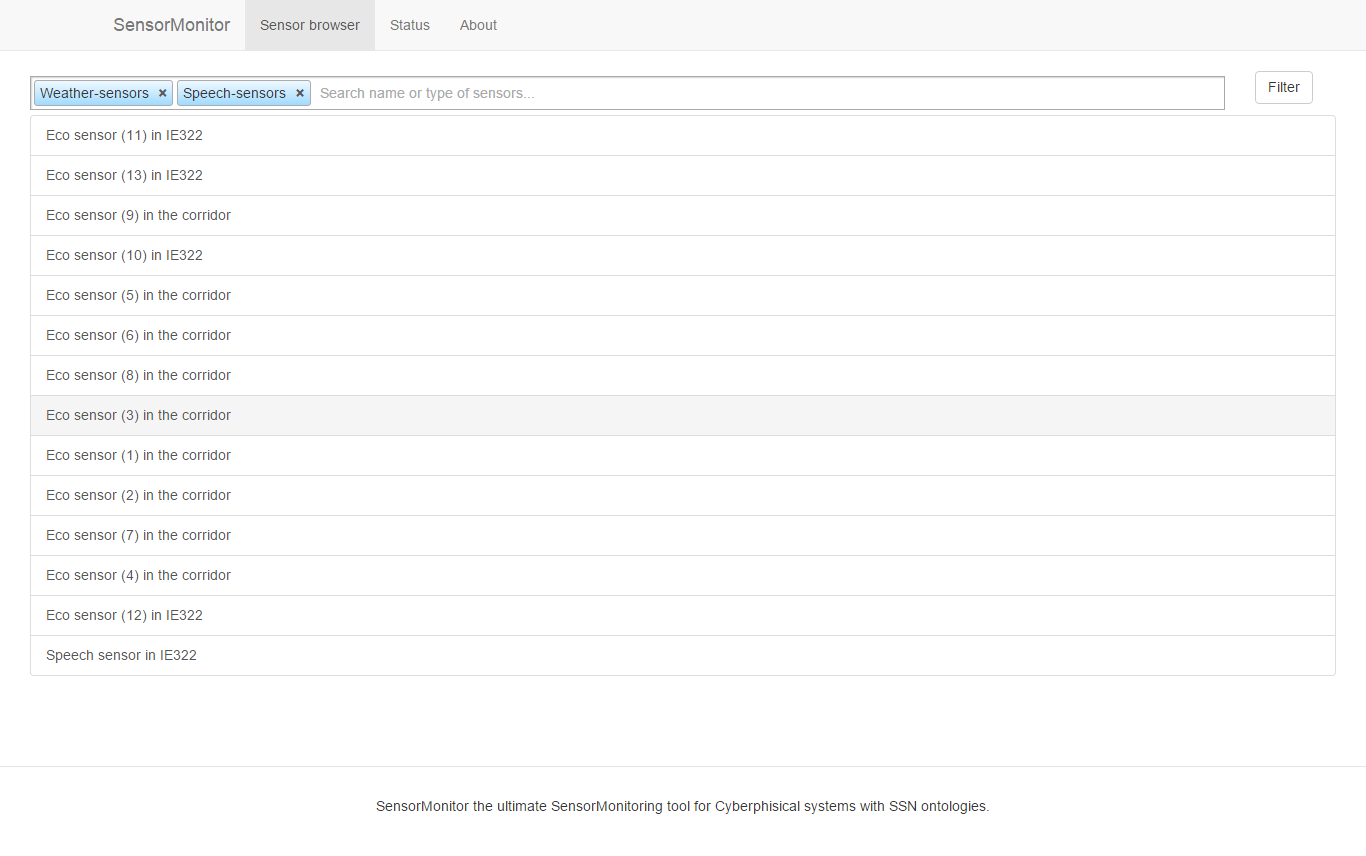
\includegraphics[width=0.9\textwidth]{figures/shbrowser.png}
\caption{Screenshot of the sensor browser page.\label{fig:shbrowser}}
\end{figure}

It is possible to filter on certain categories. For that the input field has to be used at the top of the page. By typing more than 3 letters into the field, an Autocomplete list will drop down with the possible completion of the phrase. If nothing is found, there won't be any drop down menus. The user has to click on the wanted item from the list to add a new filter condition. After selecting one or multiple filters the Filter button has to be pushed to apply the changes. The list will refresh and show the union of all the given categories. The system can not parse those items in the input field which are not selected through the list.  

\subsection{Sensor details page}
If one sensor is clicked a details page is shown for the selected sensor. The  page shows two calendars from which the first one lets the user select the start date of the shown period, the second is for the end date of the period. The data between these two dates are shown on the charts. By default the past 6 hours are selected. 

The page lists all the observed properties measured by the sensor. It can list quantities, boolean data type or text only. Quantities and boolean data is shown on a chart, while the text data is shown as a list of the messages with timestamps. The lists and charts automatically reload themselves if a different start or end time is selected. If there is no data in the given range, an error message is displayed above the chart. It will automatically disappear if the time period is changed to a range where data can be found. 

Note, that at most 50 measurements are  displayed on each chart to keep them readable.

The page also shows a map, where the current position of the sensor can be seen. The map is using Google Maps to display the data.

A screenshot can be seen on Figure \ref{fig:shshow}.

\begin{figure}[h]
\centering
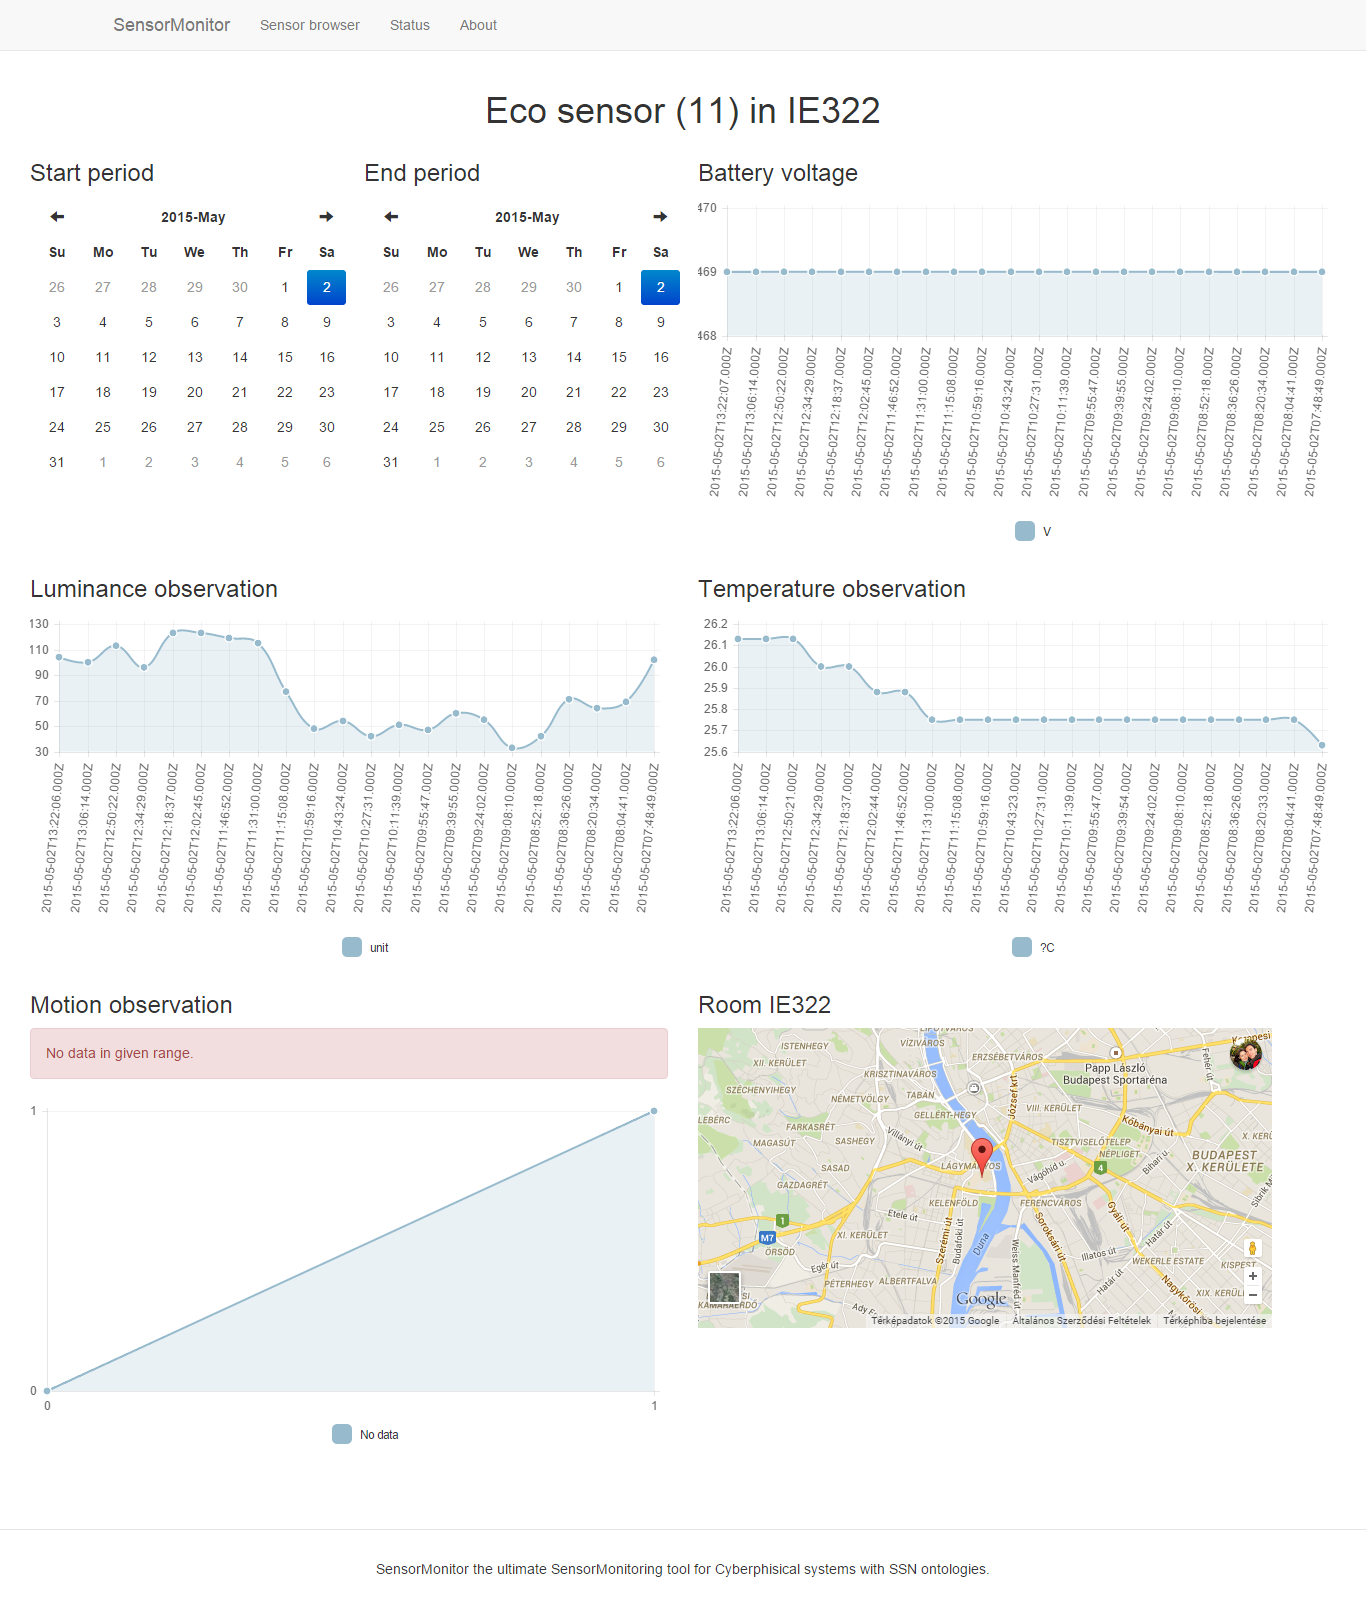
\includegraphics[width=0.9\textwidth]{figures/shshow.png}
\caption{Screenshot of the sensor details page.\label{fig:shshow}}
\end{figure}

\subsection{Status page}

The status page gives a feedback of the sensors if they are alive or no data is received from a given sensor on an observed property.

The status page shows a table of the sensor names and observed properties. If the sensor's observed property does not provide new measurements in a predefined time interval, then it is considered as down. The measurements which are down are marked with red. Those sensor's observed properties which provide new data are considered alive and they are marked with a green. 

The table can be ordered based on the observed property name or the sensor name by clicking on the headers of the table row. 

By clicking the checkbox below the title the sensors and observed properties which are alive can be hidden from the list to see the dead sources only.

The time period for checking the sensors and the time limit from which the sensor is considered dead can be set using the configuration. 

The page does not reload automatically as the time between each check should not be too often (recommended to be at least 15 minutes). The page has to be manually reloaded from time to time.

A screenshot of the page can be seen on Figure \ref{fig:shstat}.

\begin{figure}[h]
\centering
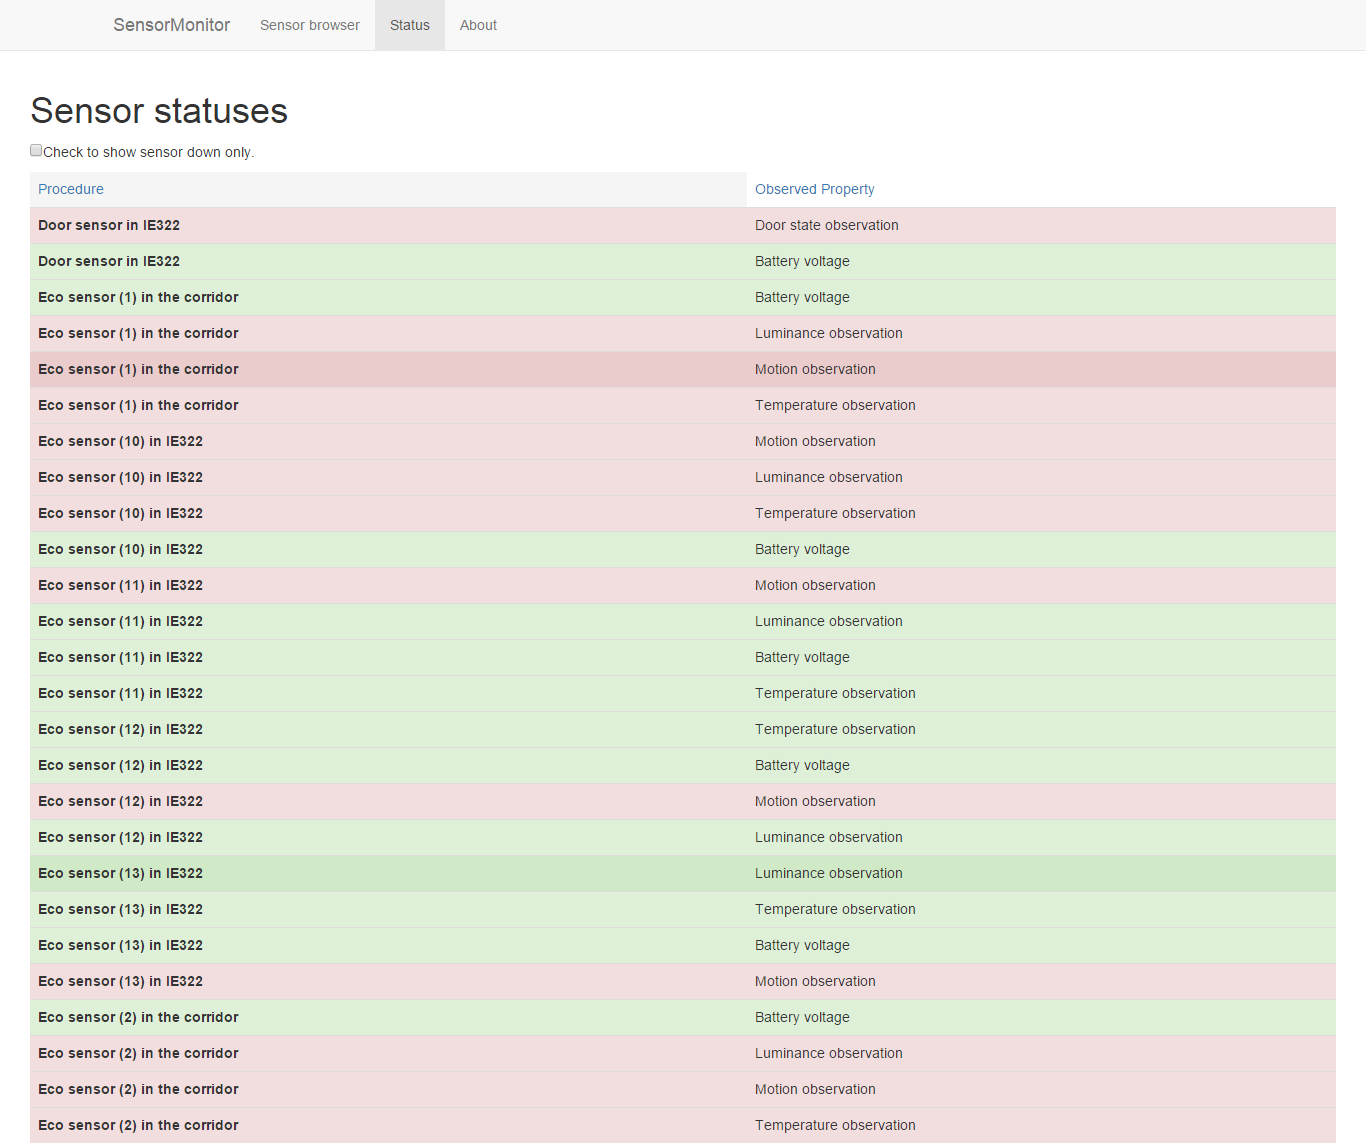
\includegraphics[width=0.9\textwidth]{figures/shstatus.png}
\caption{Screenshot of the sensor status page.\label{fig:shstat}}
\end{figure}


\subsection{Configuration of the monitoring system}
The configuration of the system can be done by editing the config files in the  server/config/environment folder. Every environment has its own configuration file, Listing \ref{lst:devconf} shows an example for the development environment. The file merges the parameters set as a JSON object with the general configuration template and returns it to the program.


\begin{lstlisting}[caption={Sample configuration for development environment\label{lst:devconf}}]
'use strict';

// Development specific configuration
// ==================================
const SPARQL_PREFIXES = "PREFIX rdf: <http://www.w3.org/1999/02/22-rdf-syntax-ns#> "+
"PREFIX owl: <http://www.w3.org/2002/07/owl#> "+
"PREFIX xsd: <http://www.w3.org/2001/XMLSchema#> "+
"PREFIX rdfs: <http://www.w3.org/2000/01/rdf-schema#> "+
"PREFIX demo: <http://mit.bme.hu/cps/demo-sensors#> " +
"PREFIX mit: <http://mit.bme.hu/cps/sensor-schema#> ";
module.exports = {
// MongoDB connection options
mongo: {
uri: 'mongodb://localhost/dipterv-dev'
},

seedDB: true,
sparql: {
host: "http://localhost:5820/",
db: "sont",
user: "admin",
pass: "admin",
prefixes: SPARQL_PREFIXES
},
sos: {
url: "http://152.66.253.152:8080/52n-sos-webapp-4.1.0/service"
},
status: {
lifetime: 60,
checkinterval: 15
}
};
\end{lstlisting}

\section{Responsiveness}

The application has been tested on multiple devices. The page load time is minimized during the build process which causes huge performance gain when loading the webpage. The page has been tested using the \url{tools.pingdom.com} website and all requests load time were under 3 seconds using a computer which ran the Windows version of the test environment. 

The website could be viewed on different screens. The content automatically scaled itself to fill the display of smaller mobile devices. For that purpose the two column structure is changed to a one column structure for the sake of readability.

\section{Future plans}

There are many ways to improve the application, because the time given limited the number of features that could be implemented. 

There can be a separate user interface for modifying the ontology and pair new values to the SOS database. Yet it is done by modifying the RDF directly and loading it into the RDF store. 

The monitoring service uses a previously implemented and extended simple ontology for the semantic connection. In the future it should be integrated with the SISRO ontology. Unfortunately in the sample system there was no connection between the two databases.

An authentication layer can be added above the system, to hide the interface from unauthorized person. As there is no database modification is done using the monitoring system this is not necessary yet. Authentication can be solved by using HTTP proxy and HTTP basic authentication on the proxy server.

The sensor list should have been filtered on multiple type. Now only the category of the sensor can be given. The system was prepared to handle multiple search criteria, it can be easily added to the system.

The load of the sensors could be displayed on the sensor list page. As the data will be stored in the RDF database, the sensor list should be able to query the load of the sensors while searching them. At the time of the writing the Sensors did not report their condition to the sample database and the scheme of the destination RDF store was different from the used ontology, which made this approach impossible.

On the sensor detail page multiple sensors data could be displayed for each observed property. The system was designed to support this function, the challenges are that the measurements are not synced on different sensors and the current chart plotter library does not support two distinct x axises in the same chart. 

More data can be displayed in each chart. The chart could contain more than 50 measurements, maybe by using a range filter or re-sampling the data somehow. There are other, non open source chart plotter libraries which seem to support this system, like HighChart.

The system could send mail alerts on status change event. The application was prepared to do that, in the status module there is a marked line where such events can be triggered. The application could log the events in a file or send an email to the administrator.

The state of each sensor should be stored in a different database. In the current system the states are stored in an array in the application, which could be a problem if the number of sensors would be greatly increased. For this reason the states should be stored in a database, perhaps in the RDF store.

The state page should also check if there is connection available to the SOS server and the RDF server to detect server failures. These errors can be detected by simply using the web page but the error messages may not be straight forward.

\section{Conclusion}
During the thesis project the author could see the steps of implementing a test environment to a cyberphisical system. Standard description format for sensor data storage of such systems got known. Databases for storing those data was investigated. The one with the most features and plarform independent implementation was chosen. The standard way to describe semantic description for such data and possible database solutions for such systems were also explained. A semantic database with great number of features and Javascript interface has been chosen. After the basics were introduced an actual use case for such a system was shown which was part of the BUTE ETIK project. The implementation of the monitoring system was based on this project. The used technologies were shared and a description of the monitoring system has been given. These technologies were NodeJS with AngularJS frontend using the previously introduced databases. 

The implementation showed that NodeJS is capable of serving the purpose of a monitoring system of Cyberphisical systems. Its great number of tools made it easy to add new features of the system. It is fast and it has great support for many interfaces. It can run with small overhead and it can be installed on most platforms. AngularJS is a great tool for Single page application, it is mobile friendly and supports most of the browsers. As web based technologies arise, this solution is a great way to write monitoring application. 

